\documentclass{IEEEtran}
\usepackage[spanish]{babel}
\usepackage[utf8]{inputenc}
\usepackage{enumerate}
\usepackage{cite}
\usepackage{graphicx}  
\usepackage{subfig}
\usepackage{float}
\usepackage{tikz}
\usepackage{pgfplots}

\usetikzlibrary{pgfplots.dateplot}
\usepackage{pgfplotstable}
\usepackage{filecontents}
\pgfplotsset{compat=1.15}
% correct bad hyphenation here
\hyphenation{op-tical net-works semi-conduc-tor}


\begin{document}
%
% paper title
% can use linebreaks \\ within to get better formatting as desired
% Do not put math or special symbols in the title.
\title{Prácticas: Difuminado de imagen}


% author names and affiliations
% use a multiple column layout for up to three different
% affiliations
\author{\IEEEauthorblockN{Andrés Fernando Román Arévalo, Ronald Sarmiento\\}
\IEEEauthorblockA{Email:afromana@unal.edu.co, roasarmientoga@unal.edu.co\\}
\IEEEauthorblockA{Universidad Nacional Bogotá, Colombia \\}
}


% make the title area
\maketitle

\nonstopmode

\tableofcontents 
\hfill


\begin{abstract}
El presente informe muestra como se llevo a cabo la paralelización  mediante el uso de distintas plataformas de programación como lo son  POSIX, openMP y CUDA   del efecto difuminado.Para un correcto analisis de los resultados se tuvo en cuenta como metricas tanto el Speed Up como de Time Response para los distintas resoluciones  de imagenes (720p, 1080p y 4k)), de kernels (2,3,4,5, 6,7, 8,9, 10,11 ,12 13 y 14) y de hilos (1,2,3,4,5,6,7,8,9 y 10)

\end{abstract}

% no keywords


\IEEEpeerreviewmaketitle



\section{Introducción.}
% no \IEEEPARstart
Una de las tareas altamente demandada en la actualidad es el procesamiento de imagenes cada vez de una mayor resolución para lo cual se requiere un alto nivel de computo. A partir de esto han surgido innumerables algoritmos que permiten paralelizar las distintas operaciones de procesamiento de imagenes como lo es la del efecto difuminado.\\\\
% You must have at least 2 lines in the paragraph with the drop letter
% (should never be an issue)
Aun asi paralelizar tiene su limite que es explicado en la Ley de Amdahl, la cual establece que hay un punto en que paralelizar ya no ofrece mejoras significativas de rendimiento e incluso por el contrario puede llevar al deterioro del mismo.\\\\

Al momento de hacer procesamiento de imagenes se utiliza distintas operaciones matriciales.En el caso del efecto borroso se realiza una convolucion entre la matriz que representa la imagen y el kernel

\begin{figure}[H]
  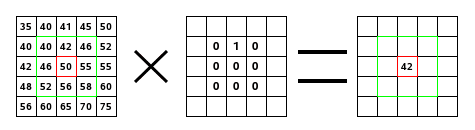
\includegraphics[width=\linewidth]{matriz.png}
  \caption{Convolucion matricial}
  \label{fig:boat1}
\end{figure}
\subsection{Creación del efecto difuminado}

Mas especificamente se utilizo la tecnica de difuminado conocida como Blur el cual consiste en intercambiar cada pixel de la imagen por un promedio de los valores RGB que se encuentras en los pixeles adyacentes a el. El nivel de difuminado esta determinado por el kernel y el tamaño da el rango que se toma para evaluar el promedio. Es decir, si se escoge un kernel de 5 significa que cada pixel sera cambiado por el promedio que hay en los promedios de la matriz 5x5 cuyo centro es el pixel en cuestion.

\section{Algoritmo de paralización.}
La paralelizacion se realizo mediante asignación tipo blockwise es decir que se tomo la imagen y se dividio a lo alto en filas y cada una de estas se asigno a un hilo. Es decir que un caso hipotetico donde se quiera aplicar el efecto difuminado a una imagen con un alto de 368 pixeles,se  lanzan 4 hilos donde el hilo 1 se le asignaba la fila 1(del pixel 0 al 92), al 2 la fila 2(del pixel 92 al 184 ), al 3 la columna 3(del pixel 184 al 276)  y al 4 la  columna 4(del pixel 276 al 368) . Para mayor clarificación detras de la idea que se uso para la paralización, la siguiente imagen:

\begin{figure}[H]
  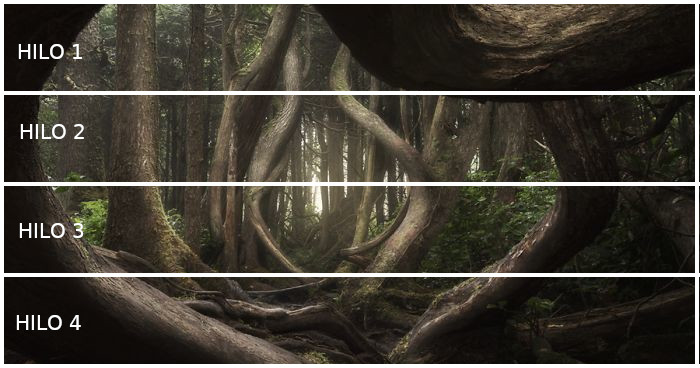
\includegraphics[width=\linewidth]{mod.jpg}
  \caption{Algoritmo de paralelización}
  \label{fig:boat2}
\end{figure}

El ejemplo anterior muestra el caso en el cual se lanza un solo bloque con 4 hilos. Lo mismo se realiza 
en las otras tecnicas de  paralelización y de computacion distribuida sino en vez de hilos se usan bloques, procesos,nodos y/o una mezcla
\section{Experimentos y resultados.}
\subsection{POSIX y OpenMP}

Antes de mostrar los resultados obtenidos y compararlos con los que se obtuvieron al paralelizar el efecto difuso con POSIX, es necesario dar a conocer las especificaciones correspondientes del ordenador donde corrio el algoritmo. Para esto se construyo la siguiente tabla resumiendo dicha información:

\begin{table}[H]
\centering
    \begin{tabular}{ |c|c| } 
\hline
\multicolumn{2}{|c|}{Especificaciones} \\
\hline
Modelo & Lenovo G50-45\\
 \hline
 Procesador & AMD A8-6410 / 2 Gz \\ 
 \hline
 Tarjeta gráfica & AMD Radeon R5 \\ 
 \hline
 Nucleos & 4\\ 
 \hline
 Memoria Ram & 8192 MB DDR3
 \\ 
 \hline
 Sistema operativo & Manjaro 18.0.4 \\ 
 \hline
\end{tabular}
\caption{Especificaciones del ordenador}
\end{table}

Para evitar o disminuir posibles interferencias se corrio un script que automaticamente cogio todos los casos de prueba mencionados en el resumen, tambien se busco que no haya ninguna aplicacion abierta mientras se corria el script

\subsubsection{Resultados}
Como primera medida se utilizo el time response o tiempo de ejecución de un programa, donde para cada imagen se crearon sus corresponientes gráficas donde en eje horizontal se colocaron el numero de hilos que ejecutaba el programa y en el eje vertical el tiempo que tardo. Para no sobrecargar la gráfica se decidio incluir solo tres nucleos por grafico, eso hace que por resolucion de imagen se crearan 2 graficos.\\
A continuacion se presentan las gráficas correspondientes:
\begin{itemize}
    \item \textbf{Imagen de 720p}
    
    \begin{tikzpicture}
\begin{axis}[
xticklabels={},
extra x ticks={1,2,4,8,16},
title={Time Response 720p},
xlabel={Numero de hilos},
ylabel={Tiempo},
nodes near coords, 
 every node near coord/.append style={font=\tiny,yshift=-1.6pt},
 nodes near coords style={/pgf/number format/.cd,precision=3},
]
\addplot coordinates { (1,0.28) (2,0.242) (4,0.213) (8,0.216) (16,0.196)  };
\addplot coordinates { (1,0.620) (2,0.397) (4,0.301) (8,0.306) (16,0.307)  };
\addlegendentry{Kernel 4}
\addlegendentry{Kernel 8}
\end{axis}
\end{tikzpicture}

\begin{tikzpicture}
\begin{axis}[
xticklabels={},
extra x ticks={1,2,4,8,16},
title={Time Response 720p},
xlabel={Numero de hilos},
ylabel={Tiempo},
nodes near coords, 
 every node near coord/.append style={font=\tiny,yshift=-1.6pt},
 nodes near coords style={/pgf/number format/.cd,precision=3},
]
\addplot coordinates { (1,0.850) (2,0.525) (4,0.392) (8,0.373) (16,0.382)  };
\addplot coordinates { (1,1.558) (2,0.833) (4,0.577) (8,0.554) (16,0.559)  };
\addlegendentry{Kernel 10}
\addlegendentry{Kernel 14}
\end{axis}
\end{tikzpicture}

\item \textbf{Imagen de 1080p}



\begin{tikzpicture}
\begin{axis}[
xticklabels={},
extra x ticks={1,2,4,8,16},
title={Time Response 1080p},
xlabel={Numero de hilos},
ylabel={Tiempo},
nodes near coords, 
 every node near coord/.append style={font=\tiny,yshift=-1.6pt},
 nodes near coords style={/pgf/number format/.cd,precision=3},
]
\addplot coordinates { (1,0.539) (2,0.385) (4,0.292) (8,0.303) (16,0.310)  };
\addplot coordinates { (1,1.34) (2,0.763) (4,0.566) (8,0.523) (16,0.545)  };
\addlegendentry{Kernel 4}
\addlegendentry{Kernel 8}
\end{axis}
\end{tikzpicture}

\begin{tikzpicture}
\begin{axis}[
xticklabels={},
extra x ticks={1,2,4,8,16},
title={Time Response 1080p},
xlabel={Numero de hilos},
ylabel={Tiempo},
nodes near coords, 
 every node near coord/.append style={font=\tiny,yshift=-1.6pt},
 nodes near coords style={/pgf/number format/.cd,precision=3},
]
\addplot coordinates { (1,1.954) (2,1.105) (4,0.698) (8,0.705) (16,0.729)  };
\addplot coordinates { (1,2.699) (2,1.515) (4,0.954) (8,0.924) (16,0.913)  };
\addplot coordinates { (1,3.587) (2,1.956) (4,1.192) (8,1.214) (16,1.223)  };
\addlegendentry{Kernel 10}
\addlegendentry{Kernel 12}
\addlegendentry{Kernel 14}
\end{axis}
\end{tikzpicture}

\item \textbf{Imagen de 4k}

\begin{tikzpicture}
\begin{axis}[
xticklabels={},
extra x ticks={1,2,4,8,16},
title={Time Response 4k},
xlabel={Numero de hilos},
ylabel={Tiempo},
nodes near coords, 
 every node near coord/.append style={font=\tiny,yshift=-1.6pt},
 nodes near coords style={/pgf/number format/.cd,precision=3},
]
\addplot coordinates { (1,4.941) (2,2.859) (4,2.245) (8,2.190) (16,2.275)  };
\addplot coordinates { (1,15.19) (2,8.295) (4,5.436) (8,5.330) (16,5.370)  };
\addlegendentry{Kernel 4}
\addlegendentry{Kernel 8}
\end{axis}
\end{tikzpicture}

\begin{tikzpicture}
\begin{axis}[
xticklabels={},
extra x ticks={1,2,4,8,16},
title={Time Response 4k},
xlabel={Numero de hilos},
ylabel={Tiempo},
nodes near coords, 
 every node near coord/.append style={font=\tiny,yshift=-1.6pt},
 nodes near coords style={/pgf/number format/.cd,precision=3},
]
\addplot coordinates { (1,22.896) (2,12.262) (4,7.750) (8,7.683) (16,7.711)  };
\addplot coordinates { (1,43.849) (2,23.408) (4,14.281) (8,13.948) (16,13.842)  };
\addlegendentry{Kernel 10}
\addlegendentry{Kernel 14}
\end{axis}
\end{tikzpicture}

\end{itemize}

Como se puede observar en las gráficas anteriores el time response del código tiene cierta tendencia de  mejorar conforme se aumenta la cantidad de hilos que son lanzados hasta los 4 hilos, de ahi en adelante la mejora es insignificante y en algunos casos como en la imagen de 720p se ve cierta desmejora.\\

Otra medida que se considero determinar para medir el rendimiento de los hilos en el programa es el speed up es decir el tiempo de ejecución secuencial dividido entre el tiempo de ejecución por cada una de las cantidad de hilos(1,2,4,8,16). \\
A continuación se presentan las gráficas correspondientes:

\begin{itemize}

\item \textbf{Imagen de 720p}

\begin{tikzpicture}
\begin{axis}[
xticklabels={},
extra x ticks={1,2,4,8,16},
title={Speed Up 720p},
xlabel={Numero de hilos},
ylabel={Tiempo},
nodes near coords, 
 every node near coord/.append style={font=\tiny,yshift=-1.6pt},
 nodes near coords style={/pgf/number format/.cd,precision=3},
 legend pos=south east,
]
\addplot coordinates { (1,1) (2,1.198347107) (4,1.361502347) (8,1.342592593) (16,1.479591837)  };
\addplot coordinates { (1,1) (2,1.561712846) (4,2.059800664) (8,2.026143791) (16,2.019543974)  };
\addlegendentry{Kernel 4}
\addlegendentry{Kernel 8}
\end{axis}
\end{tikzpicture}

\begin{tikzpicture}
\begin{axis}[
xticklabels={},
extra x ticks={1,2,4,8,16},
title={Speed Up 720p},
xlabel={Numero de hilos},
ylabel={Tiempo},
nodes near coords, 
 every node near coord/.append style={font=\tiny,yshift=-1.6pt},
 nodes near coords style={/pgf/number format/.cd,precision=3},
 legend pos=south east,
]
\addplot coordinates { (1,1) (2,1.619047619) (4,2.168367347) (8,2.278820375) (16,2.22513089)  };
\addplot coordinates { (1,1) (2,1.870348139) (4,2.70017331) (8,2.812274368) (16,2.787119857)  };
\addlegendentry{Kernel 10}
\addlegendentry{Kernel 14}
\end{axis}
\end{tikzpicture}

    \item \textbf{Imagen de 1080p}
    
\begin{tikzpicture}
\begin{axis}[
xticklabels={},
extra x ticks={1,2,4,8,16},
title={Speed Up 1080p},
xlabel={Numero de hilos},
ylabel={Tiempo},
nodes near coords, 
 every node near coord/.append style={font=\tiny,yshift=-1.6pt},
 nodes near coords style={/pgf/number format/.cd,precision=3},
 legend pos=south east,
]
\addplot coordinates { (1,1) (2,1.4) (4,1.845890411) (8,1.778877888) (16,1.738709677)  };
\addplot coordinates { (1,1) (2,1.756225426) (4,2.367491166) (8,2.562141491) (16,2.458715596)  };
\addlegendentry{Kernel 4}
\addlegendentry{Kernel 8}
\end{axis}
\end{tikzpicture}
\\
Para estas últimas tre gráficas se decidio omitir a proposito la leyenda del tiempo en cada uno de los nodos, debido a la superposicion que se genera.

\begin{tikzpicture}
\begin{axis}[
xticklabels={},
extra x ticks={1,2,4,8,16},
title={Speed Up 1080p},
xlabel={Numero de hilos},
ylabel={Tiempo},
 legend pos=south east,
]
\addplot coordinates { (1,1) (2,1.768325792) (4,2.799426934) (8,2.771631206) (16,2.680384088)  };
\addplot coordinates { (1,1) (2,1.833844581) (4,3.009228188) (8,2.954695222) (16,2.932951758)  };
\addlegendentry{Kernel 10}
\addlegendentry{Kernel 14}
\end{axis}
\end{tikzpicture}
    
\item \textbf{Imagen de 4k}\\
\begin{tikzpicture}
\begin{axis}[
xticklabels={},
extra x ticks={1,2,4,8,16},
title={Speed Up 4k},
xlabel={Numero de hilos},
ylabel={Tiempo},
 legend pos=south east,
]
\addplot coordinates { (1,1) (2,1.728226653) (4,2.200890869) (8,2.256164384) (16,2.171868132)  };
\addplot coordinates { (1,1) (2,1.831223629) (4,2.794334069) (8,2.849906191) (16,2.82867784)  };
\addlegendentry{Kernel 4}
\addlegendentry{Kernel 8}
\end{axis}
\end{tikzpicture}

\begin{tikzpicture}
\begin{axis}[
xticklabels={},
extra x ticks={1,2,4,8,16},
title={Speed Up 4k},
xlabel={Numero de hilos},
ylabel={Tiempo},
 legend pos=south east
]
\addplot coordinates { (1,1) (2,1.867232099) (4,2.954322581) (8,2.980085904) (16,2.969264687)  };
\addplot coordinates { (1,1) (2,1.873248462) (4,3.070443246) (8,3.143748208) (16,3.167822569)  };
\addlegendentry{Kernel 10}
\addlegendentry{Kernel 14}
\end{axis}
\end{tikzpicture}
    
    
\end{itemize}

Como podemos observar en las gráficas anteriores el speed up es el esperado ya que el tiempo tiene una tendencia a aumentar conforme el programa se ejecuta con más hilos.\\

Por último se considero importante realizar una comparación de time response entre el código de difuminado usando POSIX que fue el de la primera practica y el actual que es usando la librerio OpenMP. Para simplificar un poco el informe se considero solamente comparar con los kernel 6 y 12 en cada una de las resoluciones de imagen. A continuación se presentan las gráficas correspondientes:\\\\
Para estas ultimas gráficas tambien se decidio omitir la leyenda del tiempo en cada uno de los nodos, debido a la superposición que se genera.

\begin{itemize}
    \item \textbf{Imagen de 720p}
    
    \begin{tikzpicture}
\begin{axis}[
xticklabels={},
extra x ticks={1,2,4,8,16},
title={Time Response 720p},
xlabel={Numero de hilos},
ylabel={Tiempo},
]
\addplot coordinates { (1,0.450) (2,0.294) (4,0.242) (8,0.248) (16,0.245)  };
\addplot coordinates { (1,0.46) (2,0.344) (4,0.260) (8,0.262) (16,0.258)  };
\addplot coordinates { (1,1.120) (2,0.666) (4,0.453) (8,0.464) (16,0.454)  };
\addplot coordinates { (1,1.138) (2,0.691) (4,0.476) (8,0.467) (16,0.465)  };
\addlegendentry{Kernel 6 OpenMP}
\addlegendentry{Kernel 6 POSIX}

\addlegendentry{Kernel 12 OpenMP}
\addlegendentry{Kernel 12 POSIX}
\end{axis}
\end{tikzpicture}

    
\item \textbf{Imagen de 1080p}


\begin{tikzpicture}
\begin{axis}[
xticklabels={},
extra x ticks={1,2,4,8,16},
title={Time Response 1080p},
xlabel={Numero de hilos},
ylabel={Tiempo},
]
\addplot coordinates { (1,0.895) (2,0.543) (4,0.392) (8,0.393) (16,0.394)  };
\addplot coordinates { (1,0.937) (2,0.574) (4,0.408) (8,0.390) (16,0.411)  };
\addplot coordinates { (1,2.699) (2,1.515) (4,0.954) (8,0.924) (16,0.913)  };
\addplot coordinates { (1,2.709) (2,1.512) (4,0.965) (8,0.929) (16,0.944)  };
\addlegendentry{Kernel 6 OpenMP}
\addlegendentry{Kernel 6 POSIX}
\addlegendentry{Kernel 12 OpenMP}
\addlegendentry{Kernel 12 POSIX}
\end{axis}
\end{tikzpicture}


\item \textbf{Imagen de 4k}

\begin{tikzpicture}
\begin{axis}[
xticklabels={},
extra x ticks={1,2,4,8,16},
title={Time Response 4k},
xlabel={Numero de hilos},
ylabel={Tiempo},
]
\addplot coordinates { (1,9.273) (2,5.134) (4,3.574) (8,3.536) (16,3.587)  };
\addplot coordinates { (1,9.306) (2,5.169) (4,3.519) (8,3.576) (16,3.561)  };
\addplot coordinates { (1,32.137) (2,17.204) (4,10.662) (8,10.520) (16,10.426)  };
\addplot coordinates { (1,32.182) (2,17.180) (4,10.654) (8,10.556) (16,10.418)  };
\addlegendentry{Kernel 6 OpenMP}
\addlegendentry{Kernel 6 POSIX}
\addlegendentry{Kernel 12 OpenMP}
\addlegendentry{Kernel 12 POSIX}
\end{axis}
\end{tikzpicture}


\end{itemize}

Como podemos observar en las gráficas existe cierta mejora usando el equivalente de POSIX en OpenMp aunque esta mejora es más evidente en resolución de imagenes pequeñas como la de 720p.\\
La siguientes tablas ilustran lo anteriormente mencionado:\\
\begin{table}[H]
\centering
    \begin{tabular}{ |c|c|c| } 
\hline
\multicolumn{3}{|c|}{\textbf{Diferencias entre POSIX Y OpenMP}} \\
\hline
\textbf{Hilos} & \textbf{Kernel 6} & \textbf{Kernel 12}\\
\hline
1 Hilo & 0,010 & 0,018\\
 \hline
2 Hilos & 0,050 & 0,025 \\ 
 \hline
4 Hilos & 0,018 & 0,023 \\ 
 \hline
8 Hilos & 0,014 & 0,003\\ 
 \hline
16 Hilos & 0,013 & 0,011\\ 
\hline
\textbf{Promedio de diferencias} & 0,021 & 0,016\\ 
\hline
\end{tabular}
\caption{Imagen de 720p}
\end{table}

\begin{table}[H]
\centering
    \begin{tabular}{ |c|c|c| } 
\hline
\multicolumn{3}{|c|}{\textbf{Diferencias entre POSIX Y OpenMP}} \\
\hline
\textbf{Hilos} & \textbf{Kernel 6} & \textbf{Kernel 12}\\
\hline
1 Hilo & 0,042 & 0,01\\
 \hline
2 Hilos & 0,031 & -0,003 \\ 
 \hline
4 Hilos & 0,016 & 0,011 \\ 
 \hline
8 Hilos & -0,003 & 0,005\\ 
 \hline
16 Hilos & 0,017 & 0,031\\ 
\hline
\textbf{Promedio de diferencias} & 0,0206 & 0,0108\\ 
\hline
\end{tabular}
\caption{Imagen de 1080p}
\end{table}

\begin{table}[H]
\centering
    \begin{tabular}{ |c|c|c| } 
\hline
\multicolumn{3}{|c|}{\textbf{Diferencias entre POSIX Y OpenMP}} \\
\hline
\textbf{Hilos} & \textbf{Kernel 6} & \textbf{Kernel 12}\\
\hline
1 Hilo & 0,042 & 0,01\\
 \hline
2 Hilos & 0,035 & -0,024 \\ 
 \hline
4 Hilos & -0,055 & 0,011 \\ 
 \hline
8 Hilos & 0,040 & 0,036\\ 
 \hline
16 Hilos & -0,026 & -0,008\\ 
\hline
\textbf{Promedio de diferencias} & 0,0054 & 0,0082\\ 
\hline
\end{tabular}
\caption{Imagen de 4k}
\end{table}

En base a las anteriores tablas se  calcula la diferencia promedio entre la ejecución de POSIX y OpenMP en la paralelización del efecto difuminado para los kernel de 6 y 12 en el caso de la imagen de 720p es de 0,0185 segundos, en el caso de la imagen de 1080p es de 0,0157 segundos y en el caso de la imagen de 4k es de 0,0068 segundos. Por último cabe mencionar que la diferencia promedio global es de 0,01366666667 segundos

\subsection{CUDA}
Antes de mostrar los resultados obtenidos y compararlos con los que se obtuvieron al paralelizar el efecto difuso que se obtuvo con CUDA en comparación con los de CPU(POSIX Y OpenMP), es necesario decir que se corrio en el entorno de Google Colab. 


\subsubsection{Resultados}
Como primera medida se utilizo el time response o tiempo de ejecución de un programa, donde para cada imagen se crearon sus corresponientes gráficas donde en eje horizontal se colocaron el tamaño del kernel que ejecutaba el programa y en el eje vertical el tiempo que tardo.\\
A continuacion se presentan las gráficas correspondientes:
\begin{itemize}
    \item \textbf{Imagen de 720p}
    
    \begin{tikzpicture}
\begin{axis}[
xticklabels={},
extra x ticks={1,2,3,4,5,6,7,8,9,10,11,12,13,14},
title={Time Response 720p},
xlabel={Tamaño del kernel},
ylabel={Tiempo},
nodes near coords, 
 every node near coord/.append style={font=\tiny,yshift=-1.6pt},
 nodes near coords style={/pgf/number format/.cd,precision=3},
]
\addplot coordinates { (2,0.375) (3,0.355) (4,0.420) (4,0.383) (6,0.469) (7,0.396) (8,0.419) (9,0.417) (10,0.494) (11,0.492) (12,0.563) (13,0.560) (14,0.691)};
\end{axis}
\end{tikzpicture}



\item \textbf{Imagen de 1080p}

    \begin{tikzpicture}
\begin{axis}[
xticklabels={},
extra x ticks={1,2,3,4,5,6,7,8,9,10,11,12,13,14},
title={Time Response 1080p},
xlabel={Tamaño del kernel},
ylabel={Tiempo},
nodes near coords, 
 every node near coord/.append style={font=\tiny,yshift=-1.6pt},
 nodes near coords style={/pgf/number format/.cd,precision=3},
]
\addplot coordinates { (2,0.377) (3,0.372) (4,0.441) (4,0.433) (6,0.530) (7,0.526) (8,0.629) (9,0.633) (10,0.848) (11,0.845) (12,1.121) (13,1.128) (14,1.452)};
\end{axis}
\end{tikzpicture}

\item \textbf{Imagen de 4k}

    \begin{tikzpicture}
\begin{axis}[
xticklabels={},
extra x ticks={1,2,3,4,5,6,7,8,9,10,11,12,13,14},
title={Time Response 4k},
xlabel={Tamaño del kernel},
ylabel={Tiempo},
nodes near coords, 
 every node near coord/.append style={font=\tiny,yshift=-1.6pt},
 nodes near coords style={/pgf/number format/.cd,precision=3},
]
\addplot coordinates { (2,1.391) (3,1.397) (4,1.717) (5,1.734) (6,2.240) (7,2.237) (8,2.9) (9,2.898) (10,3.833) (11,3.830) (12,4.755) (13,4.768) (14,6.078)};
\end{axis}
\end{tikzpicture}


\end{itemize}

Como se puede observar en las gráficas anteriores el time response del código tiene cierta tendencia de  empeorar  conforme se aumenta el tamaño del kernel, como es el comportamiento esperado.\\
Otra medida que se considero determinar para medir el rendimiento de los hilos en el programa es el speed up que para este caso se calculo como la división entre el mejor tiempo en CPU contra con los mejores tiempos en GPU \\
A continuación se presentan las gráficas correspondientes:

\begin{itemize}
\item \textbf{Imagen de 720p}
    
\begin{tikzpicture}
\begin{axis}[
xticklabels={},
extra x ticks={4,6,8,10,12,14},
title={Speed Up 720p},
xlabel={Tamaño del kernel},
ylabel={Tiempo},
nodes near coords, 
 every node near coord/.append style={font=\tiny,yshift=-1.6pt},
 nodes near coords style={/pgf/number format/.cd,precision=3},
 legend pos=south east,
]
\addplot coordinates { (4,0.690) (6,0.978) (8,1.480) (10,1.721) (12,2) (14,2.225) };
\addplot coordinates { (4,1.480) (6,1.837) (8,2.02) (10,2.225) (12,2.467) (14,2.787) };
\addlegendentry{Speed Up GPU-CPU}
\addlegendentry{Speed Up CPU-CPU}
\end{axis}
\end{tikzpicture}
 
 \item \textbf{Imagen de 1080p}  
 
 \begin{tikzpicture}
\begin{axis}[
xticklabels={},
extra x ticks={4,6,8,10,12,14},
title={Speed Up 1080p},
xlabel={Tamaño del kernel},
ylabel={Tiempo},
nodes near coords, 
 every node near coord/.append style={font=\tiny,yshift=-1.6pt},
 nodes near coords style={/pgf/number format/.cd,precision=3},
 legend pos=south east,
]
\addplot coordinates { (4,1.245) (6,1.689) (8,2.130) (10,2.304) (12,2.408) (14,2.470) };
\addplot coordinates { (4,1.779) (6,2.277) (8,2.562) (10,2.772) (12,2.921) (14,2.955) };
\addlegendentry{Speed Up GPU-CPU}
\addlegendentry{Speed Up CPU-CPU}
\end{axis}
\end{tikzpicture}

\item \textbf{Imagen de 4k}

 \begin{tikzpicture}
\begin{axis}[
xticklabels={},
extra x ticks={4,6,8,10,12,14},
title={Speed Up 4k},
xlabel={Tamaño del kernel},
ylabel={Tiempo},
nodes near coords, 
 every node near coord/.append style={font=\tiny,yshift=-1.6pt},
 nodes near coords style={/pgf/number format/.cd,precision=3},
 legend pos=north west,
]
\addplot coordinates { (4,2.889) (6,4.140) (8,5.238) (10,5.978) (12,6.766) (14,6.467) };
\addplot coordinates { (4,2.256) (6,2.622) (8,2.850) (10,2.98) (12,3.055) (14,3.144) };
\addlegendentry{Speed Up GPU-CPU}
\addlegendentry{Speed Up CPU-CPU}
\end{axis}
\end{tikzpicture}

\end{itemize}

\subsection{OpenMPI}
Para esta practica se utilizo 2 clausters, uno que fue creado en google cloud el cual tiene 5 maquinas con las mismas configuraciones es decir con 7.5 gb de ram y 2 vcpu y otro en microsoft azure con 3.5 gb de ram y 1 solo vcpu. El algoritmo para distribuir entre maquinas utiliza MPI indicando un proceso por cada máquina del cluster(5 máquinas) y variando el numero de hilos por máquina(1 - 10) .  Se corrió el algoritmo y se sacaron las siguientes gráficas en el caso del time response:

\begin{itemize}
\item \textbf{Imagen de 720p}


\begin{tikzpicture}
\begin{axis}[
xticklabels={},
extra x ticks={1,2,3,4,5,6,7,8,9,10},
title={Time Response 720p},
xlabel={Numero de hilos},
ylabel={Tiempo},
nodes near coords, 
every node near coord/.append style={font=\tiny,yshift=-1.6pt},
    nodes near coords style={/pgf/number format/.cd,precision=3},
]
\addplot coordinates { (1,1.251) (2,1.256) (3,1.252) (4,1.215) (5,1.234) (6,1.242) (7,1.243) (8,1.238) (9,1.228) (10,1.235) };
\addplot coordinates { (1,1.238) (2,1.220) (3,1.229) (4,1.258) (5,1.213) (6,1.252) (7,1.225) (8,1.214) (9,1.24) (10,1.227) };
\addplot coordinates { (1,1.250) (2,1.260) (3,1.242) (4,1.253) (5,1.269) (6,1.294) (7,1.243) (8,1.266) (9,1.276) (10,1.251) };
\addlegendentry{Kernel 4}
\addlegendentry{Kernel 6}
\addlegendentry{Kernel 8}
\end{axis}
\end{tikzpicture}

\item \textbf{Imagen de 1080p}


\begin{tikzpicture}
\begin{axis}[
xticklabels={},
extra x ticks={1,2,3,4,5,6,7,8,9,10},
title={Time Response 1080p},
xlabel={Numero de hilos},
ylabel={Tiempo},
nodes near coords, 
every node near coord/.append style={font=\tiny,yshift=-1.6pt},
    nodes near coords style={/pgf/number format/.cd,precision=3},
]
\addplot coordinates { (1,1.281) (2,1.290) (3,1.295) (4,1.285) (5,1.276) (6,1.251) (7,1.27) (8,1.268) (9,1.212) (10,1.306) };
\addplot coordinates { (1,1.354) (2,1.336) (3,1.389) (4,1.355) (5,1.338) (6,1.374) (7,1.326) (8,1.341) (9,1.311) (10,1.276) };
\addplot coordinates { (1,1.520) (2,1.421) (3,1.466) (4,1.388) (5,1.443) (6,1.428) (7,1.409) (8,1.408) (9,1.35) (10,1.316) };

\addlegendentry{Kernel 4}
\addlegendentry{Kernel 6}
\addlegendentry{Kernel 8}
\end{axis}
\end{tikzpicture}


\item \textbf{Imagen de 4k}


\begin{tikzpicture}
\begin{axis}[
xticklabels={},
extra x ticks={1,2,3,4,5,6,7,8,9,10},
title={Time Response 4k},
xlabel={Numero de hilos},
ylabel={Tiempo},
nodes near coords, 
every node near coord/.append style={font=\tiny,yshift=-1.6pt},
    nodes near coords style={/pgf/number format/.cd,precision=3},
]
\addplot coordinates { (1,2.562) (2,2.601) (3,2.55) (4,2.568) (5,2.276) (6,2.246) (7,2.303) (8,2.281) (9,2.241) (10,2.246) };
\addplot coordinates { (1,3.151) (2,3.081) (3,3.122) (4,3.056) (5,2.832) (6,2.794) (7,2.797) (8,2.801) (9,2.81) (10,2.818) };
\addplot coordinates { (1,3.905) (2,4.060) (3,3.984) (4,3.962) (5,3.685) (6,3.677) (7,3.648) (8,3.647) (9,3.674) (10,3.718	) };

\addlegendentry{Kernel 4}
\addlegendentry{Kernel 6}
\addlegendentry{Kernel 8}
\end{axis}
\end{tikzpicture}




\end{itemize}

Al momento de graficar el speed up se comparo el de la anterior practica que fue la de CUDA con el speed up de la practica actual.  Es decir se hizo la comparación entre GPU-CPU, CPU-CPU, 1 vcpu y  2 vcpu. Las  gráficas obtenidas para los diferentes tamaños de imagenes se muestran a continuación:

\begin{itemize}
\item \textbf{Imagen de 720p}


\begin{tikzpicture}
\begin{axis}[
xticklabels={},
extra x ticks={4,6,8,10,12,14},
title={Speed Up 720p},
legend pos= north west,
xlabel={Tamaño del kernel},
ylabel={Speed Up},
]
\addplot+[nodes near coords, 
every node near coord/.append style={font=\tiny,yshift=-1.6pt},
    nodes near coords style={/pgf/number format/.cd,precision=3},] coordinates { (4,0.690) (6,0.9782) (8,1.4797) (10,1.7206) (12,2) (14,2.2547)};
\addplot+[nodes near coords, 
every node near coord/.append style={font=\tiny,yshift=-1.6pt},
    nodes near coords style={/pgf/number format/.cd,precision=3},] coordinates { (4,1.4795) (6,1.8367) (8,2.0195) (10,2.2251) (12,2.4667) (14,2.7871)};
\addplot+[nodes near coords, 
every node near coord/.append style={font=\tiny,yshift=-1.6pt},
    nodes near coords style={/pgf/number format/.cd,precision=3},] coordinates { (4,0.1578) (6,0.1956) (8,0.2372) (10,0.2846) (12,0.3254) (14,0.4497)  };
\addplot coordinates { (4,0.1321) (6,0.165) (8,0.2168) (10,0.2596) (12,0.3074) (14,0.3670)  };

\addlegendentry{GPU-CPU}
\addlegendentry{CPU-CPU}
\addlegendentry{1vcpu}
\addlegendentry{2vcpu}

\end{axis}
\end{tikzpicture} 

\item \textbf{Imagen de 1080p}


\begin{tikzpicture}
\begin{axis}[
xticklabels={},
extra x ticks={4,6,8,10,12,14},
title={Speed Up 1080p},
legend style={at={(0.97,0.5)},anchor=east},
xlabel={Tamaño del kernel},
ylabel={Speed Up},
]
\addplot+[nodes near coords, 
every node near coord/.append style={font=\tiny,yshift=-1.6pt},
    nodes near coords style={/pgf/number format/.cd,precision=3},] coordinates { (4,1.2448) (6,1.6887) (8,2.1303) (10,2.3042) (12,2.4077) (14,2.4704)};
\addplot+[nodes near coords, 
every node near coord/.append style={font=\tiny,yshift=-1.6pt},
    nodes near coords style={/pgf/number format/.cd,precision=3},] coordinates { (4,1.7789) (6,2.2773) (8,2.5621) (10,2.7716) (12,2.921) (14,2.9546)};
\addplot+[nodes near coords, 
every node near coord/.append style={font=\tiny,yshift=-1.6pt},
    nodes near coords style={/pgf/number format/.cd,precision=3},] coordinates { (4,0.2320) (6,0.308) (8,0.3974) (10,0.4982) (12,0.6123) (14,0.7192)  };
\addplot coordinates { (4,0.2085) (6,0.2540) (8,0.3283) (10,0.4448) (12,0.5837) (14,0.6989) };

\addlegendentry{GPU-CPU}
\addlegendentry{CPU-CPU}
\addlegendentry{1vcpu}
\addlegendentry{2vcpu}

\end{axis}
\end{tikzpicture} 


\item \textbf{Imagen de 4k}


\begin{tikzpicture}
\begin{axis}[
xticklabels={},
extra x ticks={4,6,8,10,12,14},
title={Speed Up 4k},
legend style={at={(0.97,0.62)},anchor=east},
xlabel={Tamaño del kernel},
ylabel={Speed Up},
]
\addplot+[nodes near coords, 
every node near coord/.append style={font=\tiny,yshift=-1.6pt},
    nodes near coords style={/pgf/number format/.cd,precision=3},] coordinates { (4,2.889) (6,4.14) (8,5.238) (10,5.978) (12,6.766) (14,6.467)};
\addplot+[nodes near coords, 
every node near coord/.append style={font=\tiny,yshift=-1.6pt},
    nodes near coords style={/pgf/number format/.cd,precision=3},] coordinates { (4,2.2562) (6,2.6224) (8,2.8499) (10,2.98) (12,3.0548) (14,3.1437)};
\addplot coordinates { (4,0.9509) (6,1.2642) (8,1.46101) (10,1.668) (12,1.856) (14,1.9795)  };
\addplot+[nodes near coords, 
every node near coord/.append style={font=\tiny,yshift=-1.6pt},
    nodes near coords style={/pgf/number format/.cd,precision=3},] coordinates { (4,1.028) (6,1.4223) (8,1.7802) (10,2.0917) (12,2.2979) (14,2.5181) };

\addlegendentry{GPU-CPU}
\addlegendentry{CPU-CPU}
\addlegendentry{1vcpu}
\addlegendentry{2vcpu}

\end{axis}
\end{tikzpicture} 




\end{itemize}


\section{Conclusiones}
\begin{enumerate}
    \item POSIX y OpemMP
            \begin{itemize}
          \item Entre mas grande es el kernel con el que se trabaja se demora un tiempo superior en realizar el efecto difuminado debido a que realiza mas operaciones al momento de calcular el promedio del kernel, haciendo que el costo computacional sea superior
          \item Como se observa en los resultados presentados en las tablas anteriores la mejora solo se aprecia que es significativa hasta los 4 hilos y considero que se debe a que el procesador donde se corrio el código  solo posee 4
          nucleos
          \item Aunque la diferencia entre el uso de POSIX y OpenMP podria parecer muy pequeña en realidad al momento de hacer un gran conjunto de  operaciónes tipo  difuminado esta puede ser considerable. Tambien hay que considerar que el algoritmo a nuestra consideración esta bastante optimizado como para que haya una diferencia mayor entre el uso de POSIX y OpenMP
        \end{itemize}
         
    \item CUDA
    
         \begin{itemize}
          \item Entre mas grande es el kernel con el que se trabaja se demora un tiempo superior en realizar el efecto difuminado debido a que realiza mas operaciones al momento de calcular el promedio del kernel, haciendo que el costo computacional sea superior
          \item Se evidencia que el speedup de GPU es menor cuando el computo a realizar es considerablemente menor, ya que es necesario tener en cuenta los tiempos de copia de los datos a calcular en el device y luego la recepcion en host, además que para la implementacion en cuestión es necesario realizar una transformacion de matrizde OpenCV a arreglo de enteros.
          \item Es necesario realizar una comparacion de las implementaciones de CPU y GPU para reconocer cual tiene mejor rendimiento, para nuestra práctica solo vale la pena usar GPU en el computo de imagenes 4K.
        \end{itemize} 
    \item OpenMPI
\end{enumerate}
    \begin{itemize}
        \item Los equipos que computan el problema son maquinas virtuales que están asignadas por google cloud, esto no necesariamente implica que las maquinas son contiguas en una LAN, lo que se asegura es que hacen parte de una misma VLAN lo cual impacta en el desempeño. 
          \item Asegurar que todas las maquinas en el cluster tienen las mismas librerias instaladas no siempre puede ser trivial, lo cual dificulta la implementación.
          \item al igual que en GPU la aceleracion aumenta en la medida que el tiempo de cómputo es cosiderablemente mayor al tiempo de transporte de la información.
          \item La grafica de speedup sufre un cambio similar al de la implementación en GPU, pero ya que la aceleracion es pequeña en comparación no es tan notoria la pendiente positiva.
          \item Es evidente que existe una aceleración de los tiempos de respuesta con respecto a la mejor implementación paralela en una sola máquina, sin embargo aun no se iguala la velocidad que alcanzó la implementación en una GPU.
    \end{itemize}

\noindent 


\begin{thebibliography}{00}
\bibitem{b2} Pedraza, C. (2019). Diapositivas de clase.
\bibitem{b1}David, K. and Wen-Mei, H. (2010). Programming massively parallel processos. 2nd ed. Morgan Kaufmann.
\bibitem{b2} Thomas, R. and Gudula, R. (2010). Parallel Programming. 1st ed. Springer.
\bibitem{b2} En.wikipedia.org. $(2019). Box blur.  Available at: https://en.wikipedia.org/wiki/Box_blur.$
\end{thebibliography}




% that's all folks
\end{document}


